

\chapter{Second Experimental Evaluation Cycle}
\label{chap:second_experiment}

This chapter describes the second experimental cycle of this research, building upon the findings of the first cycle detailed in Chapter 3. The rapid evolution of generative AI frameworks and models, along with the insights gained previously, prompted a more advanced and rigorous evaluation. This second phase employs non-agentic workflows as a baseline, introduces a more quantitative evaluation methodology, and leverages an automated assessment process based on the LLM-as-a-Judge concept \citep{Gu2025}. It's use was driven by the sheer volume of responses requiring evaluation. With four configurations, two models, and three executions for each of the 33 questions, a total of 792 responses were generated. Manually assessing this volume of data would have been impractical. Furthermore, previously used metrics like `truthfulness` had become less critical. This metric was highly relevant when models frequently hallucinated, a problem that is far less prevalent in the current generation of LLMs, shifting the focus to precision and recall of factual information.


\section{Design Science Research Framework}

    This second experimental cycle adheres to the Design Science Research (DSR) methodology, focusing on refining the artifacts and evaluation based on the outcomes of the first cycle.

    \begin{description}
        \item[Context] The operational environment of well construction engineering, where practitioners require efficient and reliable access to vast amounts of technical and ESG-related information.

        \item[Problem] The first experimental cycle revealed several limitations, including the subjective nature and scalability issues of expert-based evaluation, the need to compare agentic systems against simpler non-agentic baselines, and the challenge of ensuring consistent performance. This second cycle addresses the problem of developing a more robust, scalable, and objective method for evaluating and comparing different LLM-based architectures for domain-specific Q\&A.

        \item[Proposed Artifacts] Four distinct architectures were designed and implemented to compare different strategies for information retrieval and reasoning:
        \begin{itemize}
            \item A non-agentic \textbf{Linear-Flow} RAG pipeline.
            \item A non-agentic \textbf{Linear-Flow with a Router} to direct queries.
            \item A \textbf{Single-Agent} architecture, refined from the first experiment.
            \item A \textbf{Multi-Agent Supervisor} architecture for distributed reasoning.
        \end{itemize}

        \item[Evaluation] The artifacts are evaluated using an automated pipeline. An LLM-as-a-Judge assesses the generated answers against a ground-truth dataset. The evaluation is based on quantitative information retrieval metrics: \textbf{Precision}, \textbf{Recall}, and \textbf{F1-Score}.
    \end{description}

\section{Context and Problem Statement}

    \subsection{Context}

    As established in the previous chapters, this research is situated within the oil and gas industry, specifically in the domain of well construction and maintenance. Engineers and specialists in this field must navigate a complex information landscape, drawing from operational reports, ESG alerts, and documented best practices (Learned Lessons) to make critical decisions. The effectiveness of these decisions hinges on the speed and accuracy with which relevant information can be retrieved and synthesized.

    \subsection{Problem}

    The first experimental cycle confirmed the potential of LLM-based agents but also highlighted key challenges. The manual, expert-led evaluation process was time-consuming and difficult to scale. Furthermore, the performance differences between single and multi-agent systems suggested that a more granular analysis was needed, including a comparison with non-agentic RAG workflows to establish a performance baseline. Therefore, the central problem for this second cycle is to design and execute a more rigorous, automated, and scalable evaluation to definitively compare the efficacy of various agentic and non-agentic architectures in this specialized domain.


\section{Proposed Artifacts}

    To address the research problem, four distinct artifacts were developed, representing a spectrum of complexity from simple sequential pipelines to collaborative multi-agent systems. 
    
    \subsection{System Architecture Overview}

    The experimental system was implemented using \citet{Langchain2025} and \citet{Langgraph2025} frameworks specialized in language model orchestration. This modular design allows for the systematic and reproducible evaluation of different components and workflows. Key layers of the architecture include:

    \begin{itemize}
        \item \textbf{Experiment Orchestration:} Manages the execution loop, iterating through all combinations of questions, models, and setups.
        \item \textbf{Agent Workflow Frameworks:} Defines the logic for each of the four proposed artifacts using LangGraph to create cyclical graphs for agentic behavior.
        \item \textbf{Tool Integration:} A standardized interface providing agents with access to external knowledge sources. This layer enables consistent semantic search over domain-specific vector stores, ensuring that performance differences are attributable to architectural choices rather than variations in data access.
        \item \textbf{Prompt Engineering:} A library of system messages and prompt templates designed to guide the LLM's reasoning process for each specific task within the workflows.
        \item \textbf{State Management and Logging:} Captures the complete execution trace of each run, including intermediate steps, tool calls, and final outputs. This observability is essential for understanding not just the final output, but the process by which each architecture arrived at its answer.
    \end{itemize}


    \subsection{Artifact 1: Linear-Flow}

        The \textbf{Linear-Flow} architecture represents the simplest non-agentic RAG design, serving as a performance baseline. As shown in Figure \ref{fig:diagrama_linear_flow}, user input is processed in a strictly sequential manner. The user's query is handled by a single LLM step, which contains all the instructions needed to generate search queries for every available tool.
        
        \begin{figure}[h]
            \centering
            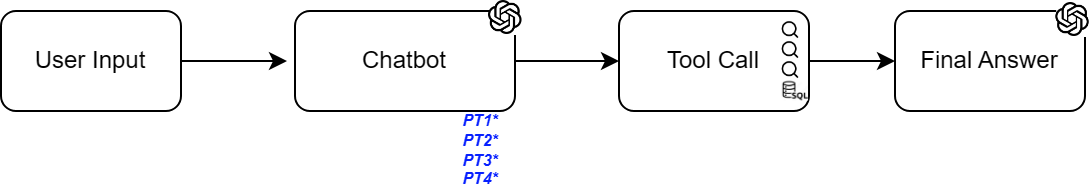
\includegraphics[width=0.8\textwidth]{images_exp2/diagrams/diagrama_linear_flow.png}
            \caption{Linear-Flow architecture. PTn indicates the prompt for Tool n.}
            \label{fig:diagrama_linear_flow}
        \end{figure}

        Because the instruction prompts for all tools are aggregated into a single call, the resulting context for the LLM becomes notably extensive and complex. While this approach is straightforward to implement, its primary drawback is the potential for performance degradation as the context length increases, which can dilute the model's focus and lead to less precise retrieval queries.
        

    \subsection{Artifact 2: Linear-Flow with Router}
    
        The \textbf{Linear-Flow with Router} paradigm (Figure \ref{fig:diagrama_linear_w_router}) extends the basic pipeline by introducing a routing mechanism to create a descentralized, non-agentic workflow. This architecture first directs a user's question to a \textbf{router node}, which is a preliminary LLM call tasked with analyzing the query and determining the most appropriate tool or sequence of tools to use.

        \begin{figure}[h]
            \centering
            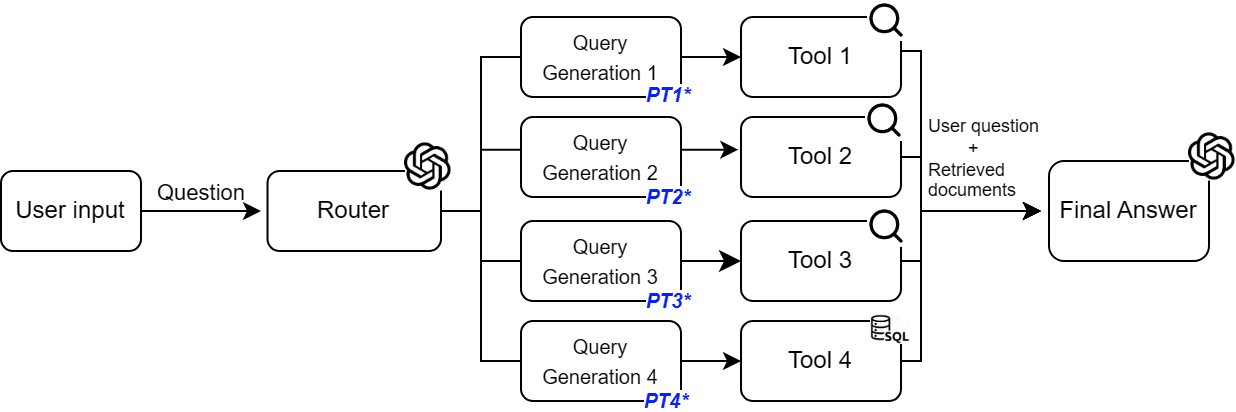
\includegraphics[width=0.8\textwidth]{images_exp2/diagrams/diagrama_linear_w_router.png}
            \caption{Linear-Flow with Router architecture.}
            \label{fig:diagrama_linear_w_router}
        \end{figure}

        This design enables the distribution of complex instruction prompts into smaller, more specialized nodes. Instead of one large prompt, several targeted sub-queries are generated, each dispatched to its respective tool. This approach offers two main advantages:

        \begin{itemize}
            \item \textbf{Specialization:} Each tool receives a query tailored to its specific function, leading to more accurate and relevant retrieval results.
            \item \textbf{Reduced Context:} By breaking down the master prompt, each LLM call operates on a smaller, more focused context, mitigating performance issues associated with long context windows.
        \end{itemize}


    \subsection{Artifact 3: Single-Agent}

        The \textbf{Single-Agent} architecture (Figure \ref{fig:diagrama_single_agent}) embodies a centralized agentic approach, building on the lessons from the first experimental cycle. In this setup, a single LLM agent manages the entire question-answering process. It has access to the full suite of tools and autonomously makes decisions about which to invoke, in what order, and how to synthesize the retrieved information into a final answer.
        
        \begin{figure}[h]
            \centering
            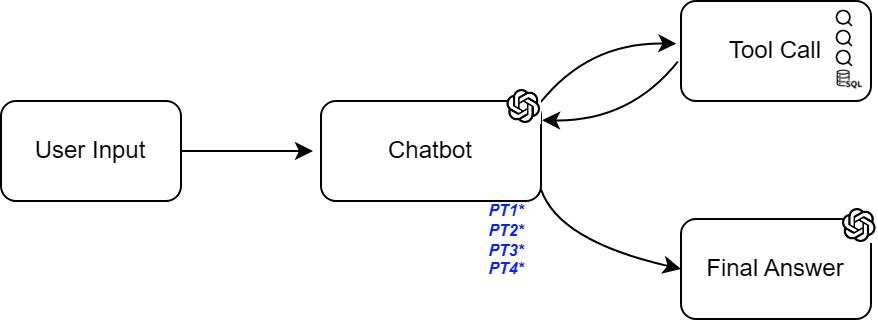
\includegraphics[width=0.5\textwidth]{images_exp2/diagrams/diagrama_single_agent.png}
            \caption{Single-Agent architecture.}
            \label{fig:diagrama_single_agent}
        \end{figure}    

        The design emphasizes \textbf{end-to-end reasoning within a unified context}, allowing the model to maintain the same ``thought process'' from start to finish. This artifact tests the capability of a standalone LLM agent to manage a RAG workflow, balancing the tool calling for different knowledge sources, all without the communication overhead required by multi-agent systems.
        

    \subsection{Artifact 4: Multi-Agent Supervisor}
    
        The \textbf{Multi-Agent Supervisor} setup (Figure \ref{fig:diagrama_multiagente_supervisor}) implements a collaborative, hierarchical system to explore the benefits of distributed cognition. This architecture consists of two main components:        

        \begin{enumerate}
            \item \textbf{A Supervisor Agent:} This master agent receives the user's query, analyzes it, and orchestrates the workflow by delegating these tasks to the appropriate specialist agents.
            \item \textbf{Specialist Agents:} A team of agents, each focusing on a specific domain of knowledge or reasoning skill. For this experiment, each specialist was tied to a single tool (e.g., a Learned Lessons Agent, an HSE Alert Agent).
        \end{enumerate}
        
        \begin{figure}[h]
            \centering
            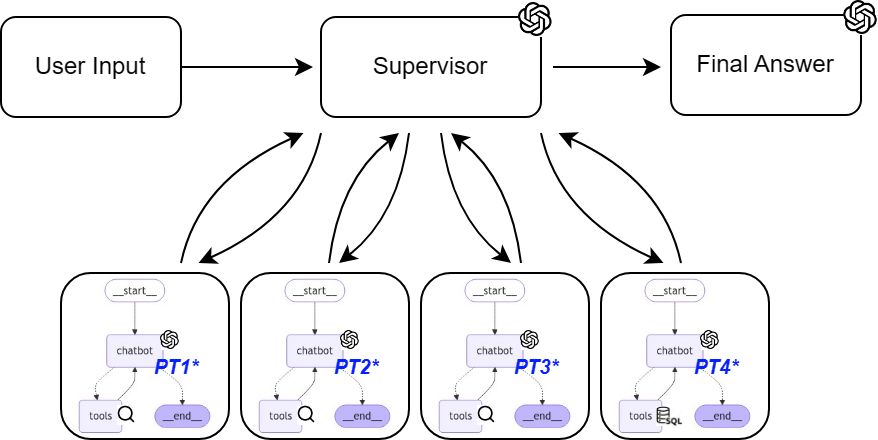
\includegraphics[width=0.6\textwidth]{images_exp2/diagrams/diagrama_multiagente_supervisor.png}
            \caption{Multi-Agent Supervisor architecture with four specialist agents.}
            \label{fig:diagrama_multiagente_supervisor}
        \end{figure}

        The supervisor orchestrates the collaboration, integrates the findings from each specialist, and synthesizes the potentially divergent information into a single, coherent final answer. This framework is designed to mimic real-world expert collaboration and tests whether decomposing a problem and assigning its parts to dedicated specialists yields a more accurate result.
        
        
\section{Evaluation}

    The evaluation phase was designed to be automated, scalable, and objective, addressing the limitations of the first experimental cycle.

    \subsection{Evaluation Methodology}

        The core of the evaluation is an automated execution loop (detailed in Algorithm \ref{alg:execution_loop}) that runs each of the 33 questions through every combination of artifact (4 setups) and model (2 models), repeating each run three times to account for stochasticity.

        \begin{algorithm}[h]
        \caption{Experiment Execution Loop}
        \begin{algorithmic}[1]
        \Require questions, setups, models
        \Ensure results
        \Function{RunExperiment}{}
            \State $results \gets \{\}$
            \ForAll{$question \in questions$}
                \State $ground\_truth \gets question.ground\_truth$
                \ForAll{$setup \in setups$}
                    \ForAll{$model \in models$}
                        \For{$i \in 1 \dots 3$} \Comment{Execute 3 times for consistency}
                            \State $agent \gets \text{InitializeAgent}(setup, model)$
                            \State $response \gets agent.\text{ProcessQuestion}(question)$
                            \State $metrics \gets \text{EvaluateResponse}(response, ground\_truth)$
                            \State Store $metrics$ and $response$ in $results$
                        \EndFor
                    \EndFor
                \EndFor
            \EndFor
            \State \Return $\text{AggregateResults}(results)$
        \EndFunction
        \end{algorithmic}
        \label{alg:execution_loop}
        \end{algorithm}

        The quality of each generated response is assessed using the LLM-as-a-Judge approach. A powerful LLM (GPT-4) is prompted to act as an impartial evaluator, comparing the generated answer against the ground-truth answer. The judge decomposes both texts into atomic statements and classifies them to build a confusion matrix, from which the final metrics are calculated. The full prompt for the LLM-as-a-Judge can be found in Appendix \ref{code:llm-judge}.

    \subsection{Data Set Creation}

        The experiment utilizes a curated dataset developed in collaboration with domain experts.
        \begin{itemize}
            \item \textbf{Questions Dataset:} A set of 17 questions reflecting real-world information needs of well engineers. Each question is paired with a manually created, expert-validated ground-truth answer.
            \item \textbf{Knowledge Bases:} The artifacts were given access to three distinct, pre-processed knowledge sources from within the organization, vectorized for semantic search:
            \begin{itemize}
                \item \textbf{Learned Lessons:} A repository of learned lessons, best practices, and operational alerts.
                \item \textbf{HSE Alerts:} A collection of ESG alerts and incident reports.
                \item \textbf{Operational Reports:} A database of detailed daily operational reports from drilling rigs.
            \end{itemize}
        \end{itemize}

    \subsection{Evaluation Metrics}

        To provide a quantitative and objective assessment, the following information retrieval metrics, detailed in Section~\ref{sec:precision_recall_f1_review}, were calculated for each response based on the LLM-as-a-Judge's analysis:
        \begin{itemize}
            \item \textbf{Precision:} Measures the accuracy of the information presented in the generated answer. It is the ratio of correct statements (True Positives) to the total number of statements made. 
            \item \textbf{Recall:} Measures the completeness of the answer. It is the ratio of correct statements retrieved to the total number of statements available in the ground truth.
            \item \textbf{F1-Score:} The harmonic mean of Precision and Recall, providing a single, balanced measure of overall performance.
        \end{itemize}

    \subsection{Results}


        To ensure a robust evaluation and account for the inherent non-determinism of language models, each of the 17 questions in the dataset was processed three times for every model and configuration combination. This experimental design resulted in a total of 408 executions (17 questions $\times$ 2 models $\times$ 4 configurations $\times$ 3 runs). Each of the 408 generated answers was then compared to a ground truth answer to calculate performance metrics.

        The results presented in this section are derived from this set of runs. For each of the 136 unique combinations of question, model, and configuration, the best-performing run (out of three) was selected based on the F1-Score. The final metrics reported in Table~\ref{tab:performance_metrics} represent the average of these best-run scores across all 17 questions for each of the eight model-configuration pairs. This approach presents a clear view of the potential of each setup, with the F1-Score serving as the primary metric for performance evaluation.

        \begin{landscape}
            \begin{table}[H]
            \centering
            \caption{Detailed performance metrics by model and agent configuration. The best result for each metric is highlighted in bold and underlined. For the inferior model, the best result is only underlined.}
            \label{tab:performance_metrics}
            % \resizebox{\textwidth}{!}{%
            \begin{tabular}{@{}llcccccccccccc@{}}
                \toprule
                \multirow{2}{*}{\textbf{Model}} & \multirow{2}{*}{\textbf{Configuration}} & \multicolumn{4}{c}{\textbf{F1-Score}} & \multicolumn{4}{c}{\textbf{Precision}} & \multicolumn{4}{c}{\textbf{Recall}} \\
                \cmidrule(l){3-6} \cmidrule(l){7-10} \cmidrule(l){11-14}
                & & Mean & Std. Dev. & Min & Max & Mean & Std. Dev. & Min & Max & Mean & Std. Dev. & Min & Max \\
                \midrule
                \multirow{4}{*}{GPT-4o} & Linear-Flow (Baseline) & 0.581 & 0.204 & 0.000 & 1.000 & 0.656 & 0.262 & 0.000 & 1.000 & 0.548 & 0.201 & 0.000 & 1.000 \\
                & Linear-Flow w/ Router & \textbf{\underline{0.702}} & 0.202 & 0.333 & 1.000 & \textbf{\underline{0.805}} & 0.185 & 0.400 & 1.000 & \textbf{\underline{0.674}} & 0.242 & 0.286 & 1.000 \\
                & Single-Agent & 0.643 & 0.213 & 0.364 & 1.000 & 0.751 & 0.198 & 0.400 & 1.000 & 0.618 & 0.240 & 0.294 & 1.000 \\
                & Multi-Agent & 0.664 & 0.214 & 0.286 & 1.000 & 0.746 & 0.221 & 0.286 & 1.000 & 0.630 & 0.231 & 0.286 & 1.000 \\
                \midrule
                \multirow{4}{*}{GPT-4o-mini} & Linear-Flow (Baseline) & 0.534 & 0.208 & 0.000 & 0.923 & 0.604 & 0.262 & 0.000 & 1.000 & 0.516 & 0.216 & 0.000 & 0.923 \\
                & Linear-Flow w/ Router & \underline{0.604} & 0.155 & 0.333 & 1.000 & 0.676 & 0.196 & 0.300 & 1.000 & \underline{0.602} & 0.206 & 0.267 & 1.000 \\
                & Single-Agent & 0.576 & 0.184 & 0.308 & 1.000 & 0.719 & 0.214 & 0.286 & 1.000 & 0.544 & 0.227 & 0.231 & 1.000 \\
                & Multi-Agent & 0.596 & 0.182 & 0.348 & 1.000 & \underline{0.687} & 0.198 & 0.400 & 1.000 & 0.578 & 0.201 & 0.235 & 1.000 \\
                \bottomrule
            \end{tabular}%
            % }
            \end{table}
        \end{landscape}


        \begin{figure}[h]
            \centering
            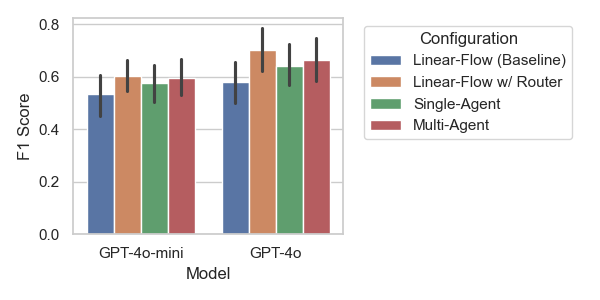
\includegraphics[width=0.7\textwidth]{images_exp2/bar_best_f1_by_model_and_configuration.png}
            \caption{Best F1-Score by model and configuration.}
            \label{fig:best_f1_by_model_and_configuration}
        \end{figure}

        
        The analysis of the results presented in Table~\ref{tab:performance_metrics} and visualized in Figure~\ref{fig:best_f1_by_model_and_configuration} reveals several insights into the performance of the different models and configurations. A primary observation is the consistent performance superiority of the GPT-4o model over its counterpart, GPT-4o-mini, across all tested configurations. The most capable configuration for GPT-4o, \textit{Linear-Flow w/ Router}, achieved a mean F1-Score of 0.702. This represents a significant performance uplift of approximately 16.2\% compared to the best score achieved by GPT-4o-mini (0.604), which was also with the \textit{Linear-Flow w/ Router} configuration. This gap underscores the impact that the model's reasoning and instruction-following capabilities have on the overall performance of the system.

        Furthermore, the results show that more complex configurations brought a notable improvement over the \textit{Linear-Flow (Baseline)} for both models. The \textit{Linear-Flow w/ Router} configuration emerged as the most effective architecture overall. For the superior GPT-4o model, this configuration boosted the mean F1-Score by a relative 20.8\% over the baseline (from 0.581 to 0.702). It also increased the mean precision by 22.7\% (from 0.656 to 0.805), indicating that the router is highly effective at selecting the correct reasoning path or tool, thereby reducing incorrect or irrelevant responses.

        While the \textit{Single-Agent} and \textit{Multi-Agent} configurations also outperformed the baseline, they did not reach the performance level of the router-enhanced linear flow. For GPT-4o, the \textit{Multi-Agent} setup (F1-Score 0.664) slightly outperformed the \textit{Single-Agent} (F1-Score 0.643), but both fell short of the \textit{Linear-Flow w/ Router}. This suggests that for the tasks in this experiment, the added complexity of reflective agent loops or multi-agent collaboration did not yield a proportional benefit over a more direct, intelligent tool-routing approach.

        A crucial aspect of the results is the high standard deviation observed across all configurations, typically around 0.20 for the F1-Score. The wide range between minimum and maximum scores indicates that performance is highly variable and question-dependent. This suggests that even the best-performing systems can fail completely on certain queries.



    \subsection{Discussion} \label{sec:exp2-discussion}

        % [DISCUSSION WILL ENTER HERE]
        The results from this second experimental cycle present a series of compelling, and in some aspects, counter-intuitive insights into the application of LLM-based architectures in specialized technical domains. The most significant finding, which stands in contrast to the prevailing trends in agentic AI and some initial findings from our first experiment, is the superior performance of a non-agentic configuration (\textit{Linear-Flow w/ Router}) over its more complex, cyclical agentic counterparts. This outcome challenges the assumption that increased agent complexity, with its capacity for reflection and iterative refinement, universally leads to better performance. This discussion will explore the primary hypothesis for this phenomenon, explore other contributing factors, and consider the broader implications for designing AI systems in niche domains.

        \subsubsection{The Domain Knowledge Deficit: Why Agentic Reflection Fails}

            The core benefit of an agentic architecture, whether single or multi-agent, lies in its ability to perform cyclical reasoning. An agent can call a tool, assess the output, reflect on its progress, and decide on a new course of action, potentially correcting earlier mistakes or refining its strategy. This iterative process is a form of simulated cognition. However, we hypothesize that the effectiveness of this reflective capability is fundamentally contingent on the LLM's pre-existing, foundational knowledge of the subject matter.
            
            For an LLM to effectively judge the output of a tool or the partial answer from a sub-agent, it must have a robust internal model of what constitutes a \textit{good} or \textit{correct} answer in that domain. Consider, for example, the domain of software engineering. LLMs like GPT-4o are extensively trained on vast repositories of code, documentation, and programming discussions. When an agent generates a piece of code, the LLM can \textit{read} it, understand its logic, identify bugs, and suggest improvements because it has been trained on countless similar examples. In this context, a cyclical, reflective flow is highly effective because the LLM is a competent judge of its own (or its peers') output.
            
            The domain of this study, well construction engineering, presents a starkly different scenario. The knowledge is highly specialized, filled with niche terminology, and often contained within proprietary corporate documents that do not form a significant part of the public web crawl used to train general-purpose LLMs. Consequently, when an agent in our experiment retrieves a technical snippet from a lessons-learned document, the LLM lacks the deep, specialized knowledge required to effectively critique it. It cannot reliably discern subtle inaccuracies, determine if the context is fully appropriate, or judge whether a sub-agent's reasoning is sound from an engineering perspective.
            
            In this context of a \textit{domain knowledge deficit}, the cyclical flow of an agentic system becomes a liability rather than an asset. The reflective loop introduces computational and cost overhead (more LLM calls, more complex state management) without a corresponding improvement in the quality of reasoning. The agent may cycle, but it does so without true insight, making the additional complexity ineffective. This leads to the observed result: the more straightforward, non-agentic approach outperforms it.
        
        \subsubsection{The Unsurprising Efficacy of Intelligent Routing}
            
            While the agentic systems underperformed, the success of the \textit{Linear-Flow w/ Router} configuration is, in itself, a significant finding. Its superior performance can be attributed to its focused efficiency. Rather than engaging in a complex, multi-step reasoning process, this architecture excels at a single, critical task: intent classification and tool selection.
            
            The initial ``router'' call is a highly targeted use of the LLM's reasoning power. Its sole purpose is to analyze the user's query and map it to the most appropriate knowledge base (tool). This is a task that even a general-purpose LLM can perform well, as it relies on semantic understanding rather than deep domain expertise. By correctly identifying the right tool from the outset, the router ensures that the subsequent retrieval step is already on the right path.
            
            This approach of ``decide once, execute well'' proved more effective for this dataset than the agents' ``execute, reflect, re-execute'' loop. It avoids the risk of error propagation inherent in cyclical systems. In an agentic loop, a minor misinterpretation in an early step can be amplified in subsequent cycles as the agent doubles down on a flawed path. The linear flow of the router configuration is immune to this, as there are no subsequent cycles to compound an error. The simplicity of its prompt and execution logic also reduces the chance of ``meta-errors'', where the LLM becomes confused by the complex state and instructions of a multi-turn agentic conversation.
        
        \subsubsection{Other Plausible Contributing Factors}
        
            Beyond the primary hypothesis of the domain knowledge deficit, several other factors likely contributed to the observed results:
            
            \begin{itemize}
                \item \textbf{Nature of the Task}: The questions in the experimental dataset, while technically complex, are primarily information retrieval tasks. They demand finding the correct facts from the knowledge base and synthesizing them into an answer. They do not necessarily require the kind of complex, multi-step deliberation or creative problem-solving where a reflective agent might theoretically excel. For such ``retrieve-and-synthesize'' queries, optimizing the retrieval step, as the router does, yields the greatest performance gain.
                
                \item \textbf{Model Capabilities (GPT-4o vs. GPT-4o-mini)}: The consistent and significant performance gap between GPT-4o and GPT-4o-mini across all configurations underscores the critical importance of the underlying model's reasoning and instruction-following capabilities. The superior performance of the \textit{Linear-Flow w/ Router} on GPT-4o (F1-Score 0.702) compared to the same configuration on GPT-4o-mini (F1-Score 0.604) highlights that even the most effective architecture is gated by the power of the engine driving it.
                
                \item \textbf{High Performance Variance}: A crucial observation is the high standard deviation across all configurations. This indicates that performance is highly dependent on the specific question being asked. Even the best-performing system failed completely on some queries (minimum F1-Score of 0.333), while succeeding perfectly on others (maximum F1-Score of 1.000). This suggests that no single architecture is a panacea. Certain query structures or topics may inherently favor one approach over another, reinforcing the conclusion that the optimal architecture is task- and domain-dependent.
            \end{itemize}
            
            In conclusion, this experiment provides strong evidence that for specialized domains where LLMs lack deep pre-existing knowledge, the architectural focus should be on optimizing the interface between the query and the external knowledge tools. A simple, intelligent routing mechanism that accurately directs a query to the correct source can be more robust and effective than a complex, cyclical agentic system that attempts to ``reason'' in a domain it does not truly understand. The assumption that more complexity equals better performance is a fallacy; true effectiveness comes from aligning the architectural design with both the nature of the task and the inherent capabilities and limitations of the language model itself.